\fancyhead[L]{\emph{EJERCICIOS DEL TEMA 1}}

\chapter*{Ejercicios de tema 1}
\addcontentsline{toc}{chapter}{Tema 1}
\large
\begin{enumerate}
    \item[$\boxed{1}$] 
    \begin{enumerate}
        \item[(a)] Reconstruya la curva en $\mathbb{R}^2$ cuya curvatura es $K(S)=1/S \ (S>0)$, efectuando las integraciones en la variable $S$ con constantes de integracion nulas  y posteriormente la reparametrización $S=\exp(t-\pi/4)$.\\
        
        \item[(b)] Calcule la longitud de arco de dicha curva entre los puntos $(1/2,-1/2)$ y $(-e^\pi/2,e^\pi/2)$.
    \end{enumerate}
    \noindent\rule{\textwidth}{0.5pt}
    (a) Dada la curva paramétrica $\mathbf{x}:\mathbb{R}\longrightarrow \mathbb{R}^2$, $\mathbf{x}(S)=(x(S),y(S))$, reconstruimos la curva como sigue:
    \begin{gather*}
        \dot{\theta}(S)=K(S)\implies \theta(S)=\int K(S) \odif{S} + \cancelto{0}{\theta_0}\\
        x(S)=\int \cos(\theta(S)) \odif{S} + \cancelto{0}{x_0} \\
        y(S)=\int \sin(\theta(S)) \odif{S} + \cancelto{0}{y_0}
    \end{gather*}
    La integral de $\theta(S)$ es inmediata: $\theta(S)=\ln{S}$, ($S>0$).
    Calculamos las integrales de $x(S),y(S)$ usando el cambio de variable $x=\ln{S}$ e integrando por \textbf{partes}:
    \begin{enumerate}
        \item[$\rightarrow$] $x(S)=\int \cos(\ln{S}) \odif{S}$
        \begin{equation*}
            \begin{split}
               x(S)=I&=\int \cos(\ln{S}) \odif{S}=I=\int \cos(x)e^x \odif{x} \\
                     &=e^x\sin(x)-\int e^x \sin(x) \odif{x}\\
                     &=e^x\sin(x)+e^x\cos(x)-\underbrace{\int e^x \cos(x) \odif{x}}_{I}\\
                     &=\frac{e^x}{2}(\cos(x)+\sin(x))\\
        \implies y(S)&=\frac{S}{2}(\sin(\ln{S})+\cos(\ln{S}))
            \end{split}
        \end{equation*}
        \item[$\rightarrow$] $y(S)=\int \sin(\ln{S}) \odif{S}$
        \begin{equation*}
            \begin{split}
               y(S)=I&=\int \sin(\ln{S}) \odif{S}=\int \sin(x)e^x \odif{x} \\
                     &=-e^x\cos(x)+\int e^x \cos(x) \odif{x}\\
                     &=-e^x\cos(x)+e^x\sin(x)-\underbrace{\int e^x \sin(x) \odif{x}}_{I}\\
                     &=\frac{e^x}{2}(\cos(x)-\sin(x))\\
        \implies y(S)&=\frac{S}{2}(\sin(\ln{S})-\cos(\ln{S}))
            \end{split}
        \end{equation*}
    \end{enumerate}
        $$
        \boxed{\mathbf{x}(S)=(S/2(\sin(\ln{S})+\cos(\ln{S})),S/2(\sin(\ln{S})-\cos(\ln{S})))}
        $$

        Si reparametrizamos la curva con el parámetro $t$, obtenemos:
        $$
        \boxed{\mathbf{x}(t)=\frac{1}{\sqrt{2}}(e^{t-\pi/4}\sin(t),e^{t-\pi/4}-\cos(t))}
        $$
        que tiene esta pinta:
        \begin{figure}[!h]
            \centering
            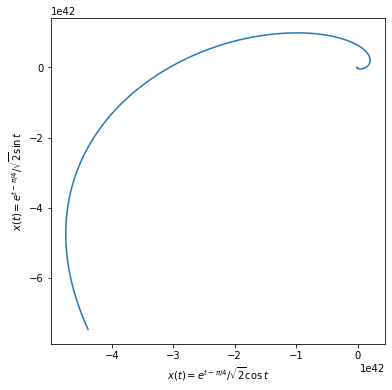
\includegraphics[scale=.5]{FOTOS/1_a.png}
            \caption*{Curva 1(a), $\mathbf{x}(t)$}
            \label{1_a}
        \end{figure}

    {\color{red} \small 10-abril-2024: Por favor, que se haga notar ese $10^{42}$ en la escala de la gráfica de la curva. El dibujo está mal (obviamente).}\\

    (b) Se puede calcular la longitud de arco en ambas parametrizaciones ya que esta es un invariante geométrico. No obstante, voy a usar la parametrización natural para aprovecharme de la propiedad de $||\dot{\mathbf{x}}(S)||=1$. La longitud de arco se calcula como:
    $$
    \ell =\int_A ^B ||\dot{\mathbf{x}}(S)|| \odif{S}=S_B-S_A
    $$

    Resolviendo el sistema de ecuaciones en cada punto, obtenemos que la $S$ debe de cumplir, en cada caso, que $\sin(\ln{S})=0$, que da soluciones periódicas de la forma $\pi k$, $k\in \mathbb{Z}$, para el logarítmo. Como estamos en $S>0$, las soluciones más próximas entre sí son $1$ y $e^\pi$, por lo que la longitud de arco es:
    $$
    \boxed{\ell=e^\pi - 1}
    $$
    \noindent\rule{\textwidth}{1pt}
    \item[$\boxed{2}$] Demuestre que la curva en $\mathbb{R}^3$ dada por $\mathbf{x}(t)=(t+ \sqrt{3}\sin t,2\cos t +2, \sqrt{3}-\sin t)$ es una hélice circular y, calculando sendos triedros de Frenet en $\mathbf{x}(0)$ y $\Tilde{\mathbf{x}}(0)$, encuentre una isometría $\Tilde{\mathbf{x}}=R\mathbf{x}+\mathbf{x}_0$ que lleve la hélice a la forma $\Tilde{\mathbf{x}}(t)=(a\cos t,a \sin t, bt)$.\\
    \noindent\rule{\textwidth}{.5pt}

    Para empezar, podemos ver que la gráfica de esta curva en $\mathbb{R}^3$ representa, efectivamente, una hélice.

    \begin{figure}[!h]
        \centering
        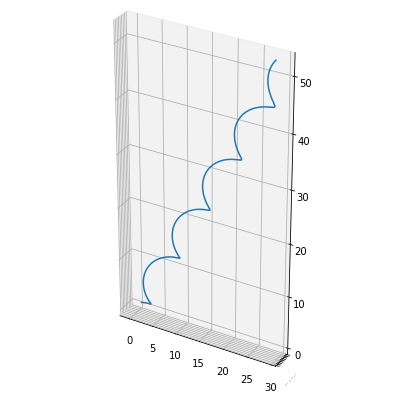
\includegraphics[scale=.5]{FOTOS/2_a.png}
        \caption*{Curva 2(a)}
        \label{fig:2a}
    \end{figure}

    Esta comienza en el punto $(0,4,0)$ y crece a lo largo de una dirección inclinada con respecto al eje vertical. En los ejemplos vistos en clase, no nos hemos encontrado en ningún momento una hélice que no tuviese como eje de simetría el eje $Z$. Por tanto, no servirá utilizar la ecuación genérica para ese tipo de hélices (que es la que proponen en el enunciado). No obstante, podremos ver que, una vez realicemos la isometría adecuada (es decir, traslaciones y rotaciones convenientes), podremos identificar la curva con la parametrización que ya conocemos. \\

    \begin{enumerate}
        \item En primer lugar, debemos demostrar que se trata de una hélice. Para ello, mostramos que la curva $\mathbf{x}(t)$ se compone de una traslación a lo largo de una dirección y de una \emph{curva plana} con radio de curvatura constante, es decir, $\rho(S)=1/K(S)\equiv$ constante. 
        \begin{equation*}
        \begin{split}
        \mathbf{x}(t)&=(t+ \sqrt{3}\sin t,2\cos t +2, \sqrt{3}-\sin t)\\
                 &=(t,2,\sqrt{3}t) \ +\ \underbrace{(\sqrt{3}\sin t,2\cos t, -\sin t)}_{\mathbf{a}(t)}
        \end{split}
        \end{equation*}

        Como habíamos enunciado, el primer término de nuestra curva es tan solo una traslación (término lineal en $t$) a lo largo de la dirección $(1,2,\sqrt{3})$. \\

        Ahora nos centramos en el siguiente término del vector. Para demostrar que se trata de una curva plana, lo más sencillo es comprobar que su \emph{vector binormal} es constante, y posteriormente calcular su radio de curvatura y ver que también es constante. \\
        Primero calculamos su primer vector del triedro de Frenet:
        $$
        \mathbf{e}_1=\frac{\mathbf{a'}(t)}{||\mathbf{a'}(t)||}=\mathbf{a'}(t)\cdot 1/2=1/2\left (\sqrt{3}\cos t,-2\sin t,-\cos t\right )
        $$
        El vector binormal $\mathbf{b}$ se obtiene como:
        $$
        \mathbf{b}(t)=\frac{\mathbf{x'}(t)\wedge \mathbf{x''}(t)}{||\mathbf{x'}(t)\wedge \mathbf{x''}(t)||}=1/4 \left ( -2,0,-2\sqrt{3} \right )\equiv \text{const.}
        $$

        Por último, la curvatura se calcula como $K=\frac{||\mathbf{x'}(t)\wedge \mathbf{x''}(t)||}{||\mathbf{x'}(t)||^3}=\frac{4}{8}=1/2$. Por tanto, el radio de curvatura es $\boxed{\rho(t)=2}$. Al tener una curva plana (vector binormal constante en la dirección de la traslación) con radio de curvatura constante, concluimos que se trata de una circunferencia y, por lo tanto, la curva parametrizada completa es una hélice.\\
        
        \textit{[Corrección]} $\mathbf{x}(t)=(t+ \sqrt{3}\sin t,2\cos t +2, \sqrt{3}-\sin t)$.\\
        
        \fbox{\parbox{4.5cm}{\textit{Hélice circular}:\\ Curva de $\mathbb{R}^3$ con sus dos curvaturas \textbf{constantes}.}} $K=\frac{w_{12}}{||\mathbf{x}'||} \ , \ \tau=\frac{w_{23}}{||\mathbf{x}'||}$
    \end{enumerate}
    \noindent\rule{\textwidth}{1pt}
    \item[$\boxed{3}$] Considere la curva $\mathbf{x}(t)=\left ( \frac{4}{5}\cos t,1-\sin t,-\frac{3}{5}\cos t \right )$. Demuestre que es una circunferencia y calcule su radio, su centro y la ecuación cartesiana del plano en que se encuentra.\\
    \noindent\rule{\textwidth}{0.5pt}
    Una circunferencia es una curva \emph{plana}, que tiene la condición de que su vector $\mathbf{b}(t)$ tiene que ser \emph{constante} para cualquier valor de $t$. Entonces, el procedimiento va a ser el siguiente:
    \begin{enumerate}
        \item Comrpobar que estamos en parametrización natural (para aliviar cálculos).
        \item Calcular $\mathbf{b}(t)$ junto con el triedro de Frenet y probar que es constante.
        \item Hallar la ecuación del plano con el vector $\mathbf{b}(t)$.
        \item Calcular su radio de curvatura y ver que es constante.
    \end{enumerate}

    En primer lugar, comprobamos que $||\mathbf{x'}(t)||=1$ (parámetro natural):
    \begin{flalign*}
        \mathbf{x'}(t)&=\left ( -\frac{4}{5}\sin t,-\cos t ,\frac{3}{5}\sin t \right ) &&\\
        ||\mathbf{x'}(t)||^2&=\frac{16}{24}\sin^2 t+\cos^2 t+\frac{9}{5}\sin^2 t=\sin^2 t+\cos^2 t\equiv 1 \smiley&&\\\\
        \implies &\text{Estamos en parametrización natural.}
    \end{flalign*}

    Ahora, calculamos los vectores del triedro de Frenet:
    \begin{flalign*}
        \dot{\mathbf{x}}(S)&=\left ( -\frac{4}{5}\sin S,-\cos S ,\frac{3}{5}\sin S \right )\equiv \mathbf{t}(S)&&\\
        \ddot{\mathbf{x}}(S)&=\left ( -\frac{4}{5}\cos S,\sin S ,\frac{3}{5}\cos S \right )&&\\\\
        \implies K(S)&=||\ddot{\mathbf{x}}(S)||=1=\rho (S) \qquad \text{(el radio de curvatura es constante)}&&\\
        \iff \mathbf{b}(S)&=\frac{\dot{\mathbf{x}}(S)\wedge \ddot{\mathbf{x}}(S)}{||\dot{\mathbf{x}}(S)\wedge \ddot{\mathbf{x}}(S)||}=\left ( -\frac{3}{5},0,-\frac{4}{5} \right )\equiv \text{const.}
    \end{flalign*}

    Es decir, que la curva es plana y su radio de curvatura es constante. Por tanto, se trata de una circunferencia. El centro de curvatura es el centro de esta circunferencia,
    $$
    \mathbf{x}_{cc}=\mathbf{x}(S)+\frac{1}{K(S)}\underbrace{\mathbf{p}(S)}_{=\mathbf{b}\wedge \mathbf{t}}=\left ( -\frac{4}{5}\cos S,\sin S ,\frac{3}{5}\cos S \right )
    $$

    La circunferencia vive en el plano \emph{perpendicular} a $\mathbf{b}(S)=\left ( -\frac{3}{5},0,-\frac{4}{5} \right )$. El plano tendrá por ecuación:
    $$
    ((x,y,z)-\overbrace{(0,0,0)}^{\in \mathbf{x}(S)})\cdot \mathbf{b}=0\implies \boxed{-3x+4z=0}
    $$

    \begin{center}
        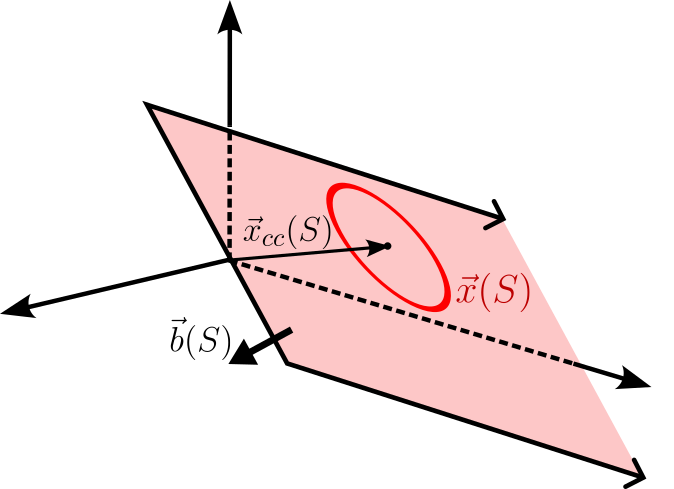
\includegraphics[scale=.5]{FOTOS/3_dibujo.png}
    \end{center}
\end{enumerate}


